\section{Results}\label{sec:results}

Muons and beam-related background  were produced by the 11 GeV electron beam interaction with the beam-dump and propagated in the region of interest as described in  Sec.~\ref{sec:sampling}.



\subsection{Muons}
Fig.~\ref{fig:mu-comp} shows the muon flux crossing the BDX-Hodo  as obtained by GEMC and FLUKA  in the  three locations of interest (A, B and C).
The flux has been sampled assuming the BDX-Hodo centred  to the beam height  Results are reported for muons generated at high statistic by the custom $\mu$ event generator and propagated using GEMC (green points in the figure).
The number of event generating at the dump correspond to  (1.2 $\pm$0.1) 10$^{12}$ EOT that correspond to a  0.2 uA 
\begin{figure}[h!] 
\center
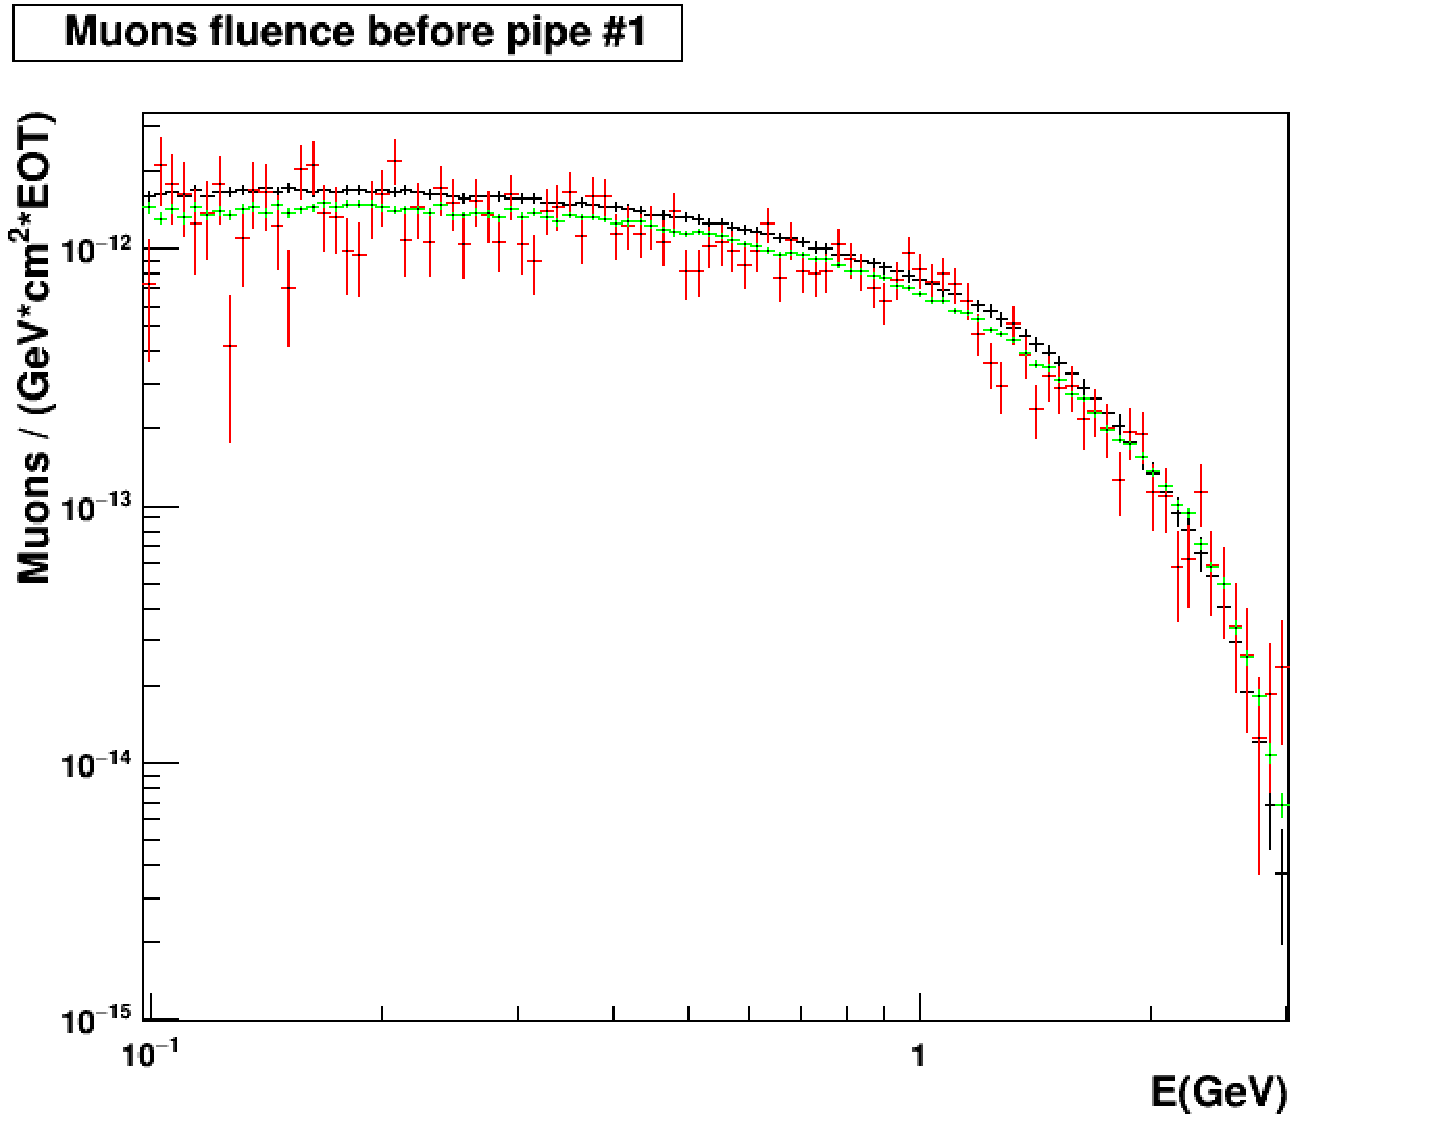
\includegraphics[width=4.7cm]{figs/comparisonMuonsPipe1_1D.pdf}
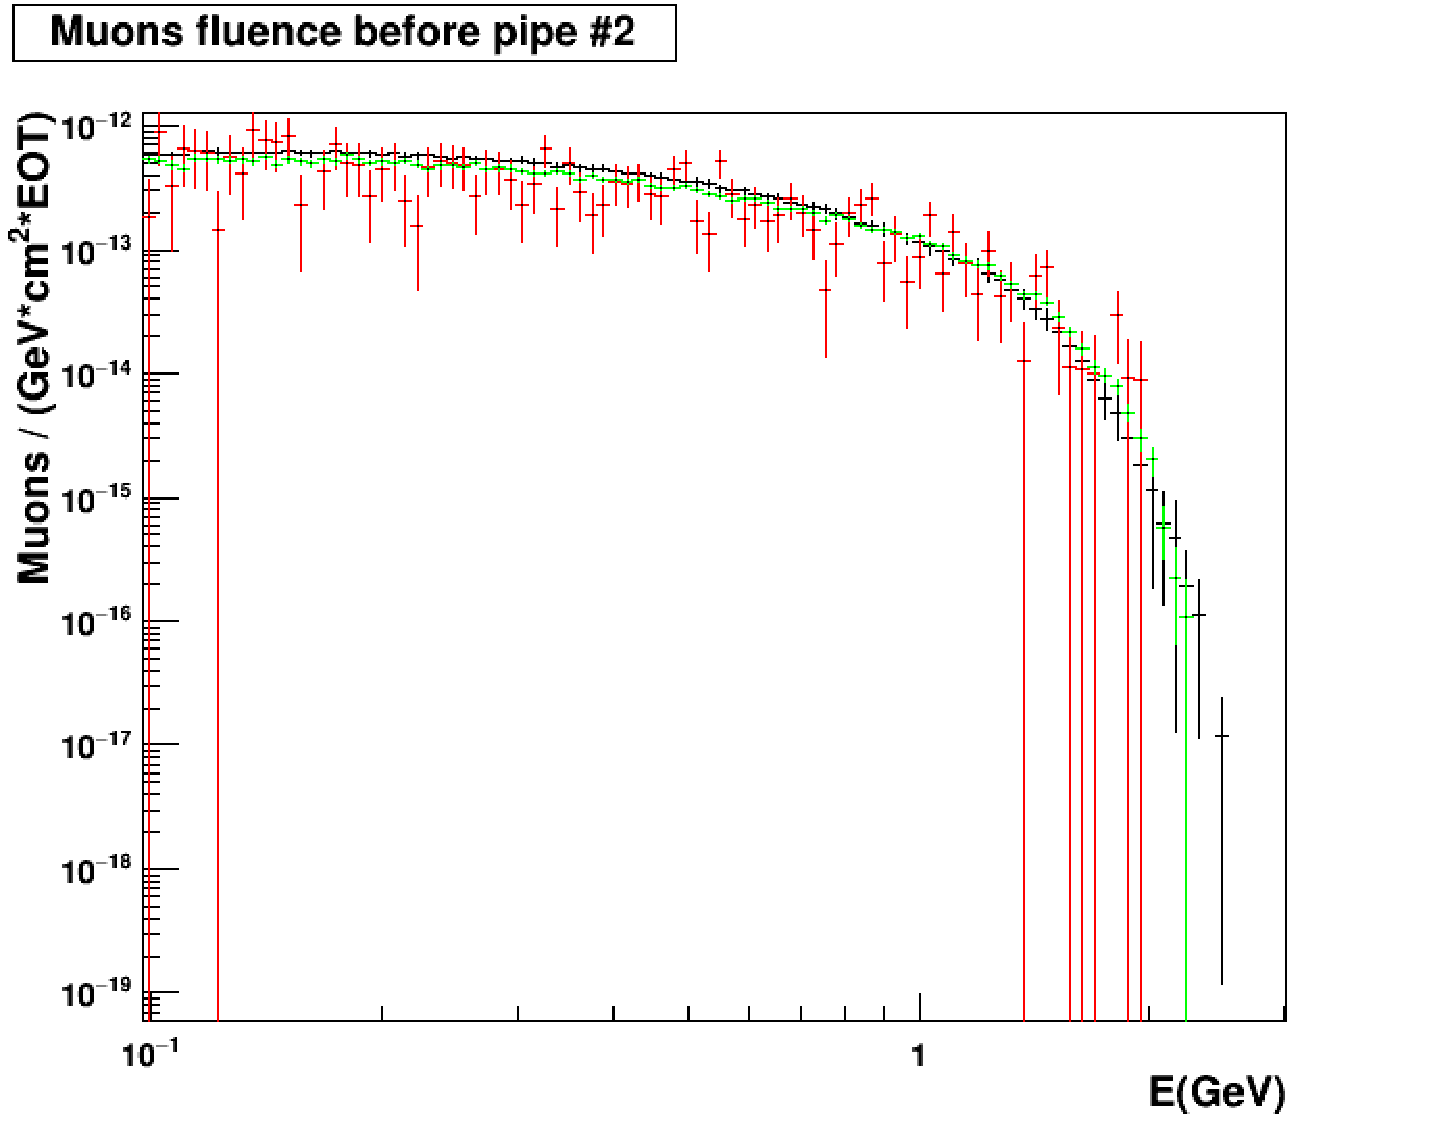
\includegraphics[width=4.7cm]{figs/comparisonMuonsPipe2_1D.pdf}
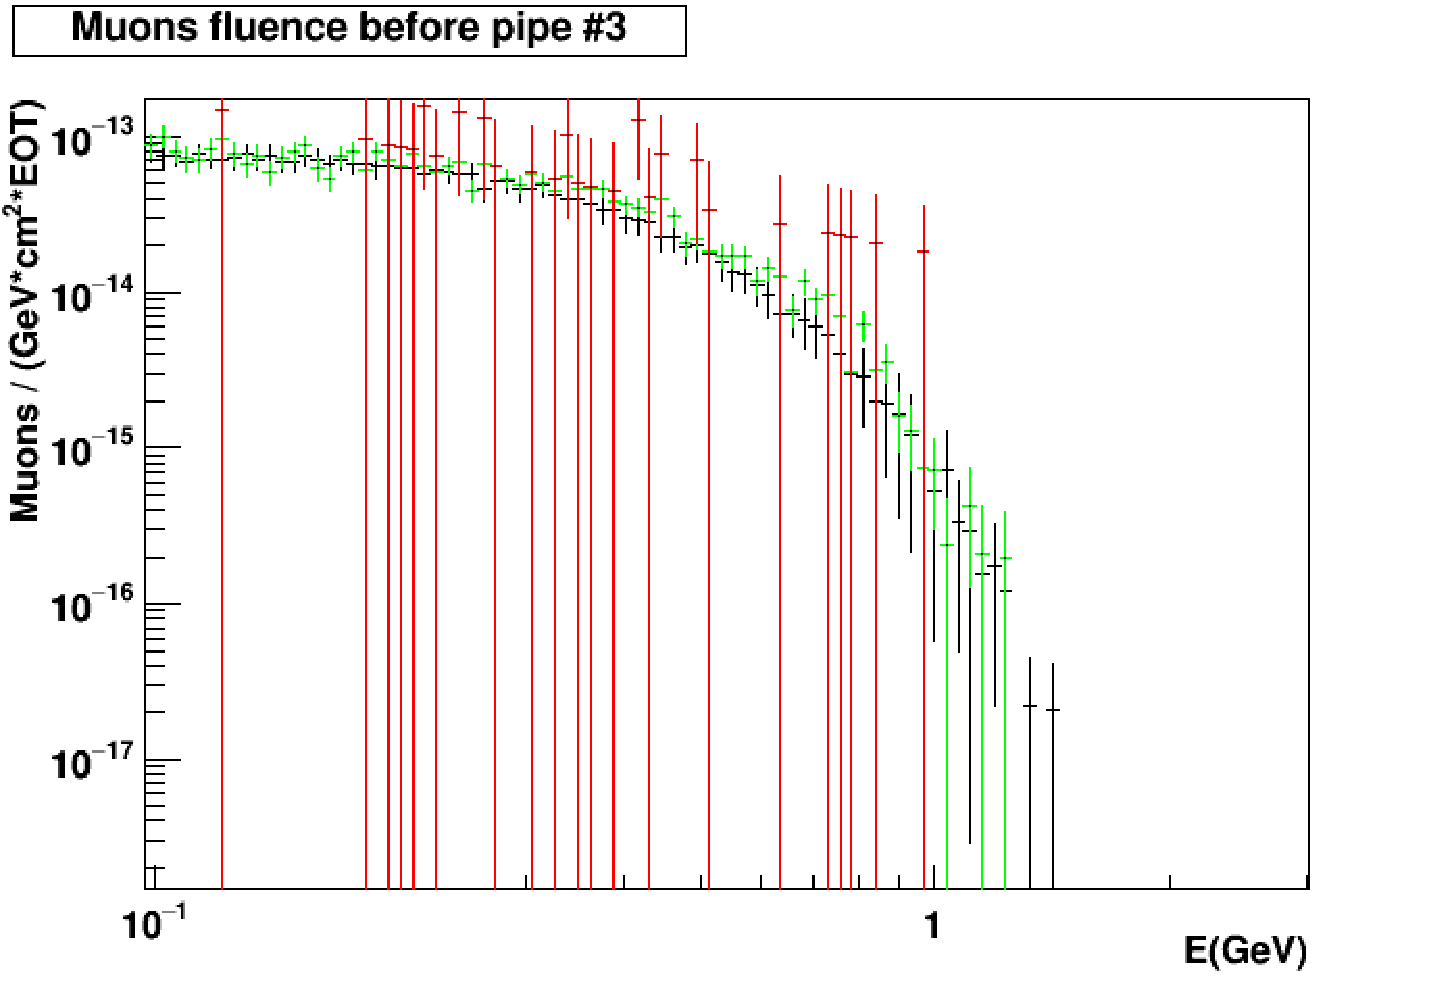
\includegraphics[width=5.5cm]{figs/comparisonMuonsPipe3_1D.pdf}
\caption{Muons energy spectra at the three locations of interest. Beam/dump interaction using  FLUKA (black), GEMC (red) and the high statistic custom $\mu$ event generator with GEMC propagation (green).}
\label{fig:mu-comp}
\end{figure}

\subsection{Muons above the ground}
For sake of completeness the muon flux has also been evaluated in the closest locations accessible above the  beam-dump vault.  This set-up assumed to positioning the detector above-the-ground not requiring any drill and simplifying the logistic of the tests.
 Due to the CPU-time necessary to track muons at such large angle (with respect to the beam axis) we used a two steps procedure. Firstly, the 11 GeV electron beam was let interact with the beam dump and muons produced on the roof of the vault has been sampled in three different position.
A high statistic sample of muons have then been generated according to the previous distributions and propagated to the outside.  Applying  a conservative hypothesis (the muons are propagated perpendicular to the beam axis  crossing the minimal amount of concrete and dirt) muons with energy higher than 4.5 GeV (the minimum to not been ranged out)  were propagated and sampled in the three perpendicular locations outdoor.


\subsubsection{Beam-related background}
Fig.~\ref{fig:nu-comp} shows the neutron flux  as obtained by  FLUKA starting from the electron/beam-dump interaction  in the  three locations of interest. 
\begin{figure}[h!] 
\center
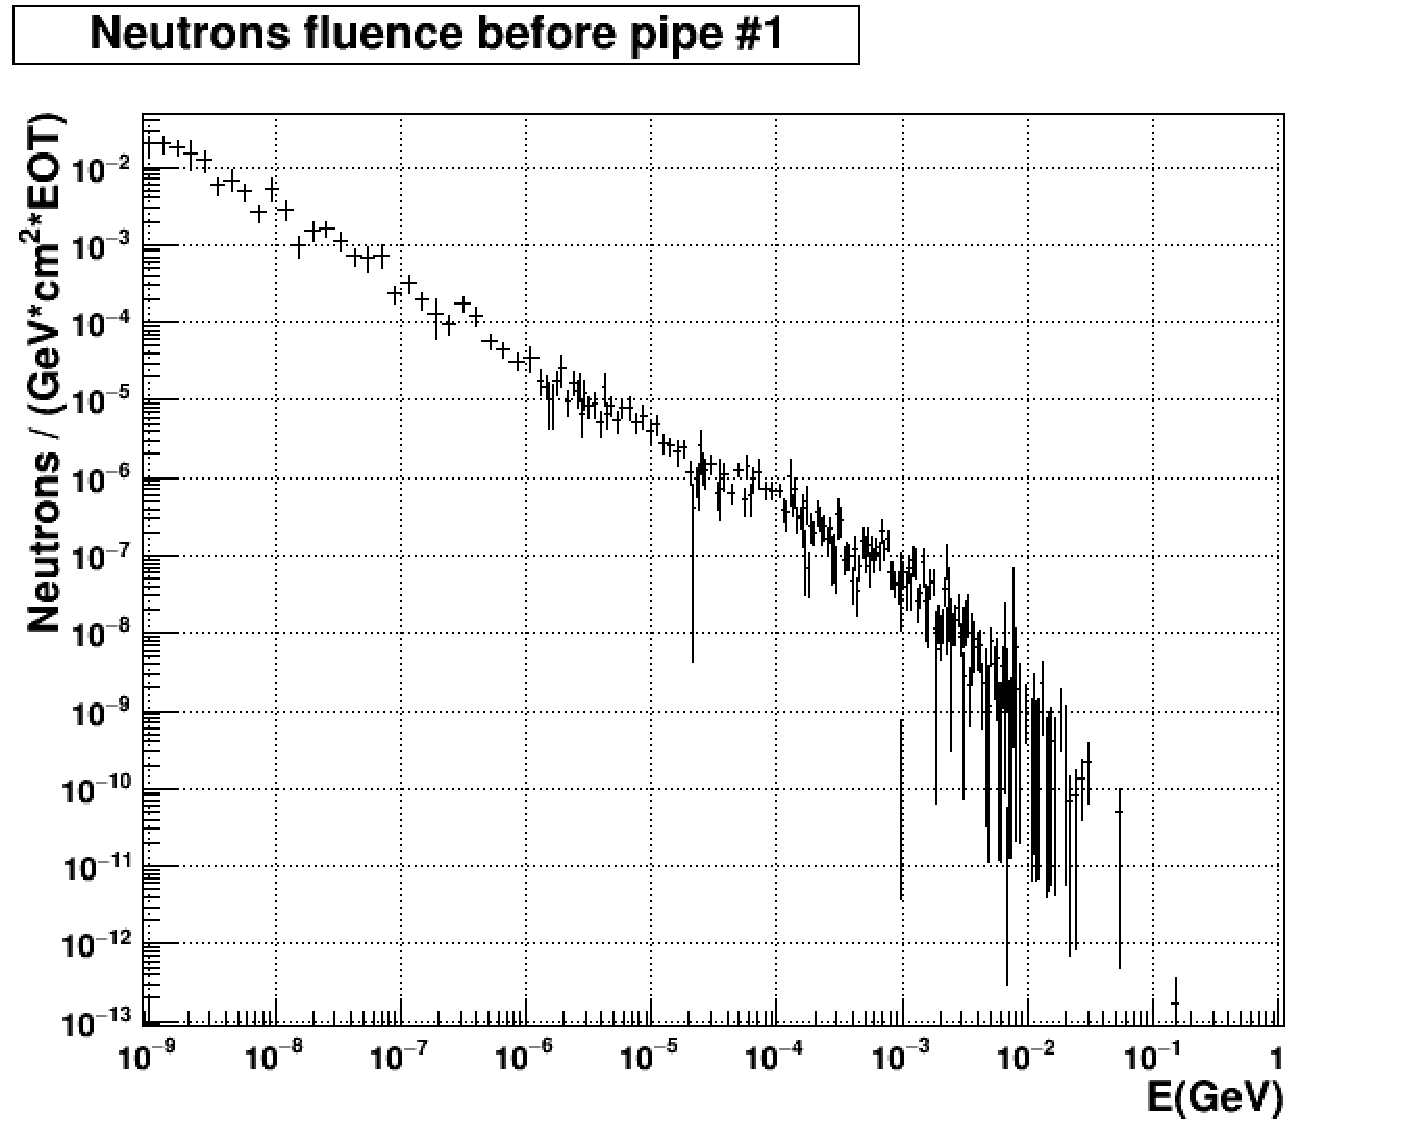
\includegraphics[width=4.7cm]{figs/NeutronsPipe1_1D.pdf}
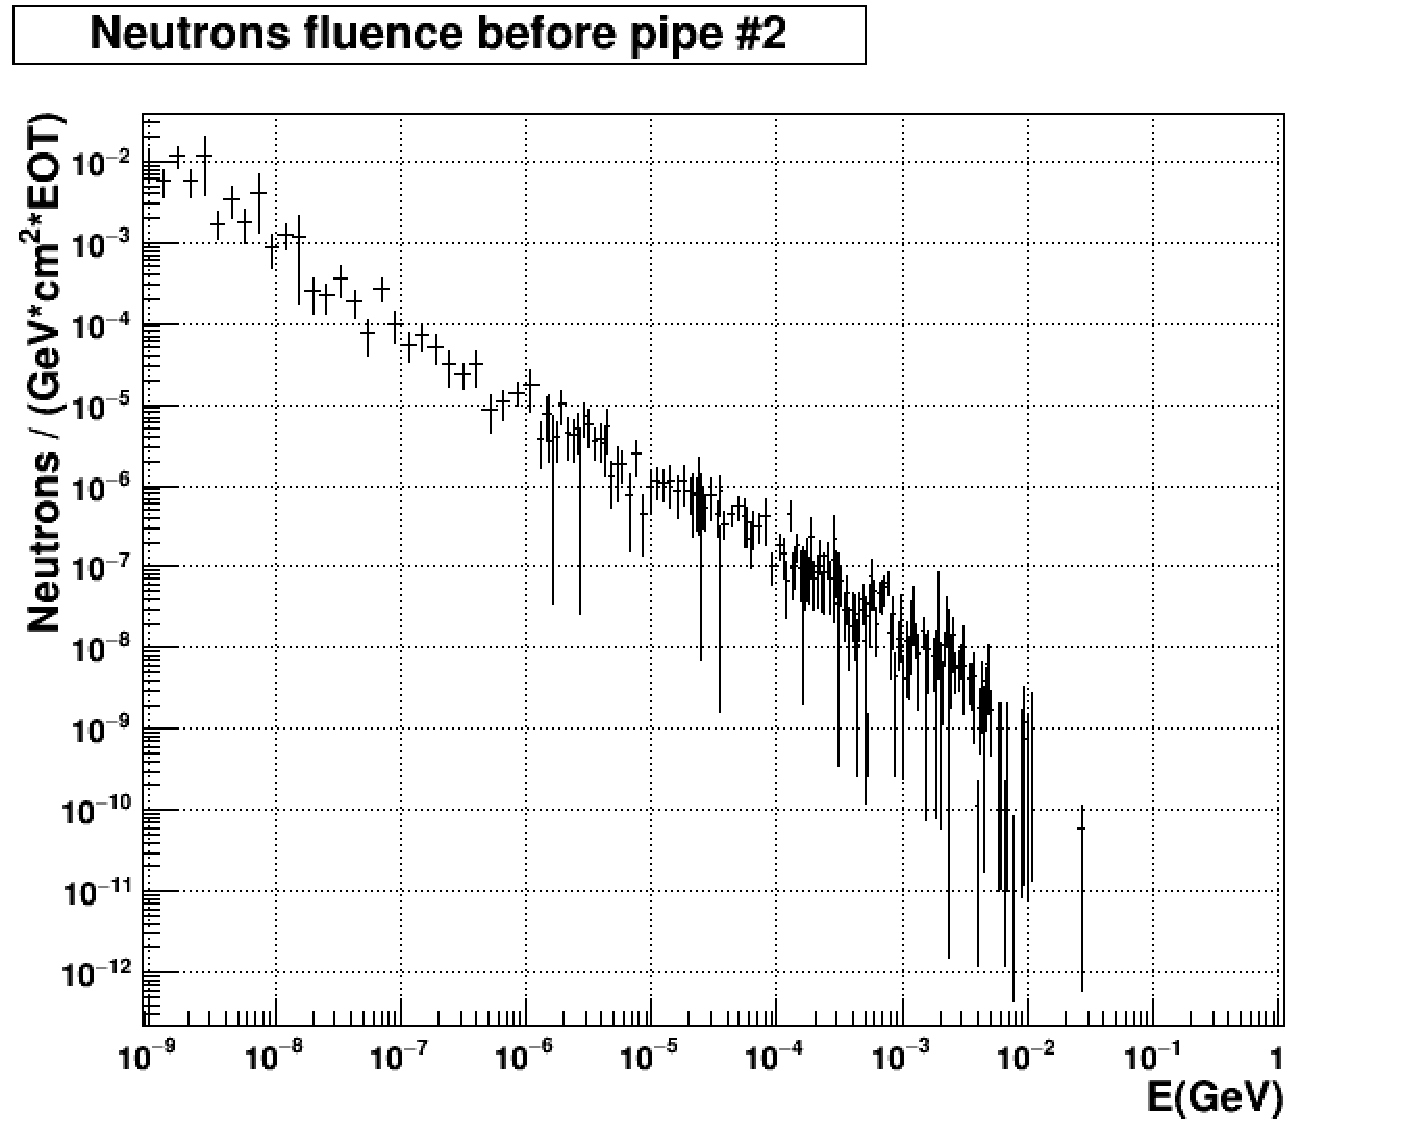
\includegraphics[width=4.7cm]{figs/NeutronsPipe2_1D.pdf}
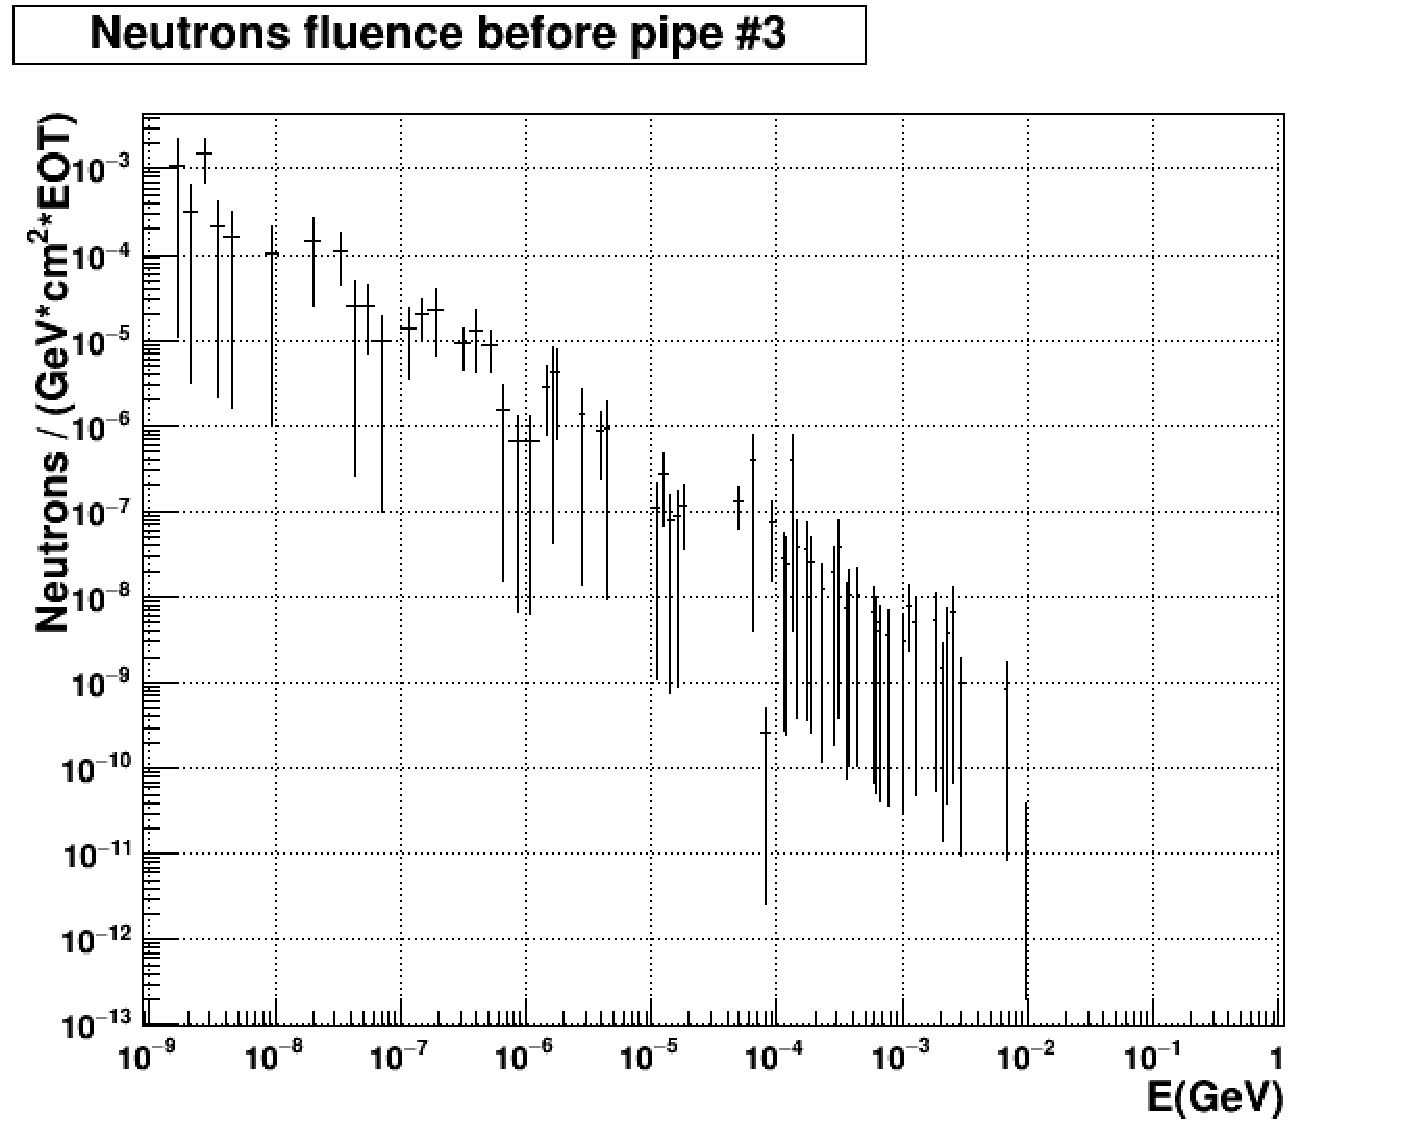
\includegraphics[width=5.5cm]{figs/NeutronsPipe3_1D.pdf}
\caption {Neutron energy spectra at the three locations of interest. Spectra are obtained from electron beam interaction with the beam-dump using FLUKA.}
\label{fig:nu-comp}
\end{figure}


\subsubsection{Cosmic background}
The cosmic muon background in the BDX-Hodo has been evaluated using GEMC. This is the same cosmic flux generator used in PR-16-001~\cite{bdx-proposal}. The muon spectrum has been divided in different ranges  and correctly weighted to estimate the full rate expected on the detector. Rates in the detector have been evaluated for CsI(Tl) crystal alone, Top scintillator alone (showing the maximum rate) and requiring  the coincidence of the front/back scintillator with the crystal (the condition used to identify and count muons produced in the beam-dump). Detection thresholds were set to  10 phe and 100 phe for scintillators and CsI. Tab.~\ref{tab:cosmic} shows the results of this study. The cosmic rate is negligible (in every condition $<$ 1 Hz) well below the expected rate of muons from the beam-dump.

\begin{table}[htp]
\caption{Cosmic rate expected in different components of BDX-Hodo}
\begin{center}
\begin{tabular}{|c|c|c|c|}
\hline
Energy range  (GeV) & Rate_{Crystal}  (Hz)&  Rate_{Top\,Scintillator} (Hz) & Rate_{Coincidence} (Hz) \\
\hline\hline
 0.2 - 2 $ & 0.01 &  0.02 & 0\\
 \hline
 2 - 10 $ & 0.2 &  0.25 & 0.01\\
 \hline
 10 - 100 $ & 0.35 &  0.4 & 0.01\\
\hline\hline
Cosmic muon rate $ & 0.56 &  0.67 & 0.02 \\
\hline\hline
\end{tabular}
\end{center}
\label{tab:cosmic}
\end{table}%


\subsection{The test configuration}
